\section{Realtime Specialization}
\label{sec:realtime}

% \subsection{Overview and Challenges}
The StepAudio 2.5 foundation is specialized into three branches: an ASR branch, a TTS branch, and the realtime spoken interaction branch detailed in this section. \steprealtime\ inherits the core foundation architecture without modification---an audio encoder, an audio adaptor that projects acoustic representations into the decoder's hidden space, and a large decoder that produces an explicit latent reasoning trace before generating a response.

Targeting multi-turn spoken interaction under stringent latency constraints introduces distinct challenges compared to standard speech-to-text tasks:
\begin{itemize}
    \item \textbf{Conversational Coherence:} Maintaining topical context, stylistic coherence, and dialogue state across extended interactions.
    \item \textbf{Persona Consistency:} Adhering to specific personality traits and delivery styles under diverse and adversarial user inputs.
    \item \textbf{Paralinguistic Sensitivity:} Understanding and appropriately responding to non-verbal cues such as hesitation, laughter, sighs, and pacing changes.
    \item \textbf{Reward Sparsity:} Unlike discrete QA tasks, conversational attributes (e.g., naturalness, emotional fit) lack a single ground-truth target, making them difficult to optimize solely via verifiable reward signals.
\end{itemize}
To address these challenges, we introduce a specialized training pipeline relying on data composition and a staged optimization recipe, without structural changes to the architecture.

\subsection{Training Pipeline}
The training pipeline systematically instills conversational capabilities while preserving the foundation model's perceptual and reasoning abilities. It consists of three main stages: audio-centric mid-training, multi-stage Supervised Fine-Tuning (SFT), and Reinforcement Learning from Human Feedback (RLHF).

\subsubsection{Audio-Centric Mid-Training}
Inherited directly from the foundation model, this phase equips the model with robust audio-grounded perception and long-form reasoning capabilities. It serves as the baseline before dialogue-specific behaviors are introduced.

\subsubsection{Progressive Supervised Fine-Tuning (SFT)}
\label{sec:realtime_sft}
The SFT phase serves as the primary vehicle for transforming the base model into a natural conversationalist. Rather than treating this as a monolithic training step, we adopt a progressive curriculum that systematically injects interactive capabilities across three core dimensions:

\begin{itemize}
    \item \textbf{Conversational Alignment:} The model is first calibrated for multi-turn interactions. Using instruction-rich dialogue data, we train it to maintain turn-level continuity, handle spoken-language artifacts (e.g., disfluencies, mid-utterance interruptions), and favor colloquial, prosody-friendly responses over formal text.
    \item \textbf{Persona and Stylistic Control:} To support diverse interaction archetypes, we introduce scalable, persona-conditioned data. By expanding a curated seed into a massive feature matrix of personality traits and verbal habits, we train the policy to condition jointly on persona specifications and dialogue history. This enables compositional generalization, allowing the model to adapt its delivery descriptors and non-verbal vocalizations (e.g., laughter, sighs) to unseen persona combinations.
    \item \textbf{Paralinguistic Sensitivity:} Using real spoken interactions, the model is trained to recognize subtle paralinguistic cues. It learns to register these cues in its latent reasoning trace and dynamically adjust its response tone and pacing. Consequently, the model synthesizes the static external persona (\emph{who is speaking}) with real-time paralinguistic reading (\emph{how the user is speaking}).
\end{itemize}

To prevent catastrophic forgetting and stylistic drift as these capabilities are introduced, we employ a \textbf{dynamic rehearsal schedule}. Throughout the SFT phase, interaction-specific data is continuously interleaved with general-purpose instruction data and reasoning tasks based on validation metrics, ensuring the model retains its foundational reasoning while mastering complex dialogue behaviors.

\subsubsection{RLHF with Generated Rewards}
To bridge the residual gap in dialogue quality where no single SFT demonstration is optimal, we apply RLHF using a PPO-style objective~\citep{schulman2017proximal} with KL regularization. A generative reward model scores candidates against reference responses, utilizing explicit interaction rubrics to guide instruction-sensitive aspects, while standard preference comparisons govern overall conversational naturalness.

Training is conducted on a mixture of multi-turn dialogues and single-turn prompts: multi-turn data encourages the policy to maintain consistency across exchanges, while single-turn prompts provide capacity for longer-form reasoning and richer preference articulation. Preference comparisons serve as the primary reward signal, capturing overall response quality. Rubric scores complement this signal on instruction-sensitive aspects, particularly those where consistency matters most, including maintaining coherence across turns and remaining faithful to earlier user content. Unlike conventional scalar reward models, the generative reward model captures finer-grained aspects of human preference, providing a richer training signal for policy alignment.

\subsection{Data}
The SFT data for \steprealtime\ is organized into three complementary streams that mirror the staged objective in Section~\ref{sec:realtime_sft}. The conversational backbone consists of multi-turn dialogues drawn from natural spoken interaction, filtered to favor turn-to-turn continuity, elliptical or disfluent phrasing, and mid-utterance revisions, with written-style responses down-weighted so that the policy is anchored to a spoken register.

Layered on top is persona-conditioned dialogue at scale. Starting from more than 10{,}000 native personas authored end-to-end and validated by human reviewers, an algorithmic fission procedure recombines orthogonal attributes—personality, verbal habits, emotional boundaries, and interaction archetypes—into a million-scale persona matrix, and each synthesized persona is paired with dialogues drawn from a million-scale real-scenario corpus so that persona attributes are grounded in realistic interaction contexts.

A third stream exposes the model to paralinguistic cues. These dialogues carry an atmosphere descriptor that governs speaking rate, stress, and subtext, alongside cue labels covering hesitation, light laughter, sigh, breath, change of pace, and falling intonation. Interleaved throughout is a general-capability mixture inherited from mid-training that preserves reasoning ability, and the full corpus passes through a unified pipeline that checks in-character consistency, cross-validates annotations, and removes near-duplicates introduced by fission.

\subsection{Evaluation}

Because realtime interaction quality depends on properties that transcript-level metrics do not capture, we evaluate \steprealtime\ in a fully interactive setting that combines subjective human evaluation conducted through mobile-app sessions with objective API-based evaluation across general dialogue, in-car dialogue, dialogue understanding, and audio-question answering. The five suites are:
\begin{itemize}
    \item \textbf{Step-Dialogue-Human-Eval}: Subjective mobile-app evaluation for general dialogue scenarios.
    \item \textbf{step\_Dialogue\_general}: Objective API evaluation for general dialogue.
    \item \textbf{step-Dialogue-car}: Objective API evaluation for in-car dialogue scenarios.
    \item \textbf{Step-Dialogue-Understanding}: 87 diverse audio samples testing the model's ability to infer speaker acoustic features (e.g., age, gender, speech rate) directly from the audio signal.
    \item \textbf{Step-SPQA}: An 11-category audio-question/audio-answer benchmark introduced in Step-Audio 2.
\end{itemize}

% \begin{table}[htbp]
% \centering
% \small
% \caption{Realtime interaction evaluation. Higher is better. Best results are in bold.}
% \label{tab:realtime_eval}
% \begin{adjustbox}{max width=\textwidth}
% \begin{tabular}{lccccc}
% \toprule
% & \multicolumn{1}{c}{Subjective (mobile-app)} & \multicolumn{4}{c}{Objective (API)} \\
% \cmidrule(lr){2-2}\cmidrule(lr){3-6}
% Model & step\_Dialogue\_human\_eval & step\_Dialogue\_general & step\_Dialogue\_car & Step-Dialogue-Understanding & Step-SPQA \\
% \midrule
% DouBao Realtime-202604 & 70.70 & 62.61 & 75.69 & 16.09 & 33.80 \\
% Gemini live-202604     & 67.16 & 76.51 & 79.40 & 58.05 & 63.20 \\
% GPT-realtime-1.5       & 68.01 & 81.60 & 80.80 & 80.46 & 53.20 \\
% \steprealtime          & \textbf{80.41} & \textbf{86.36} & \textbf{84.80} & \textbf{82.18} & \textbf{79.80} \\
% \bottomrule
% \end{tabular}
% \end{adjustbox}
% \end{table}

\begin{figure}[h]                                    
\centering                               
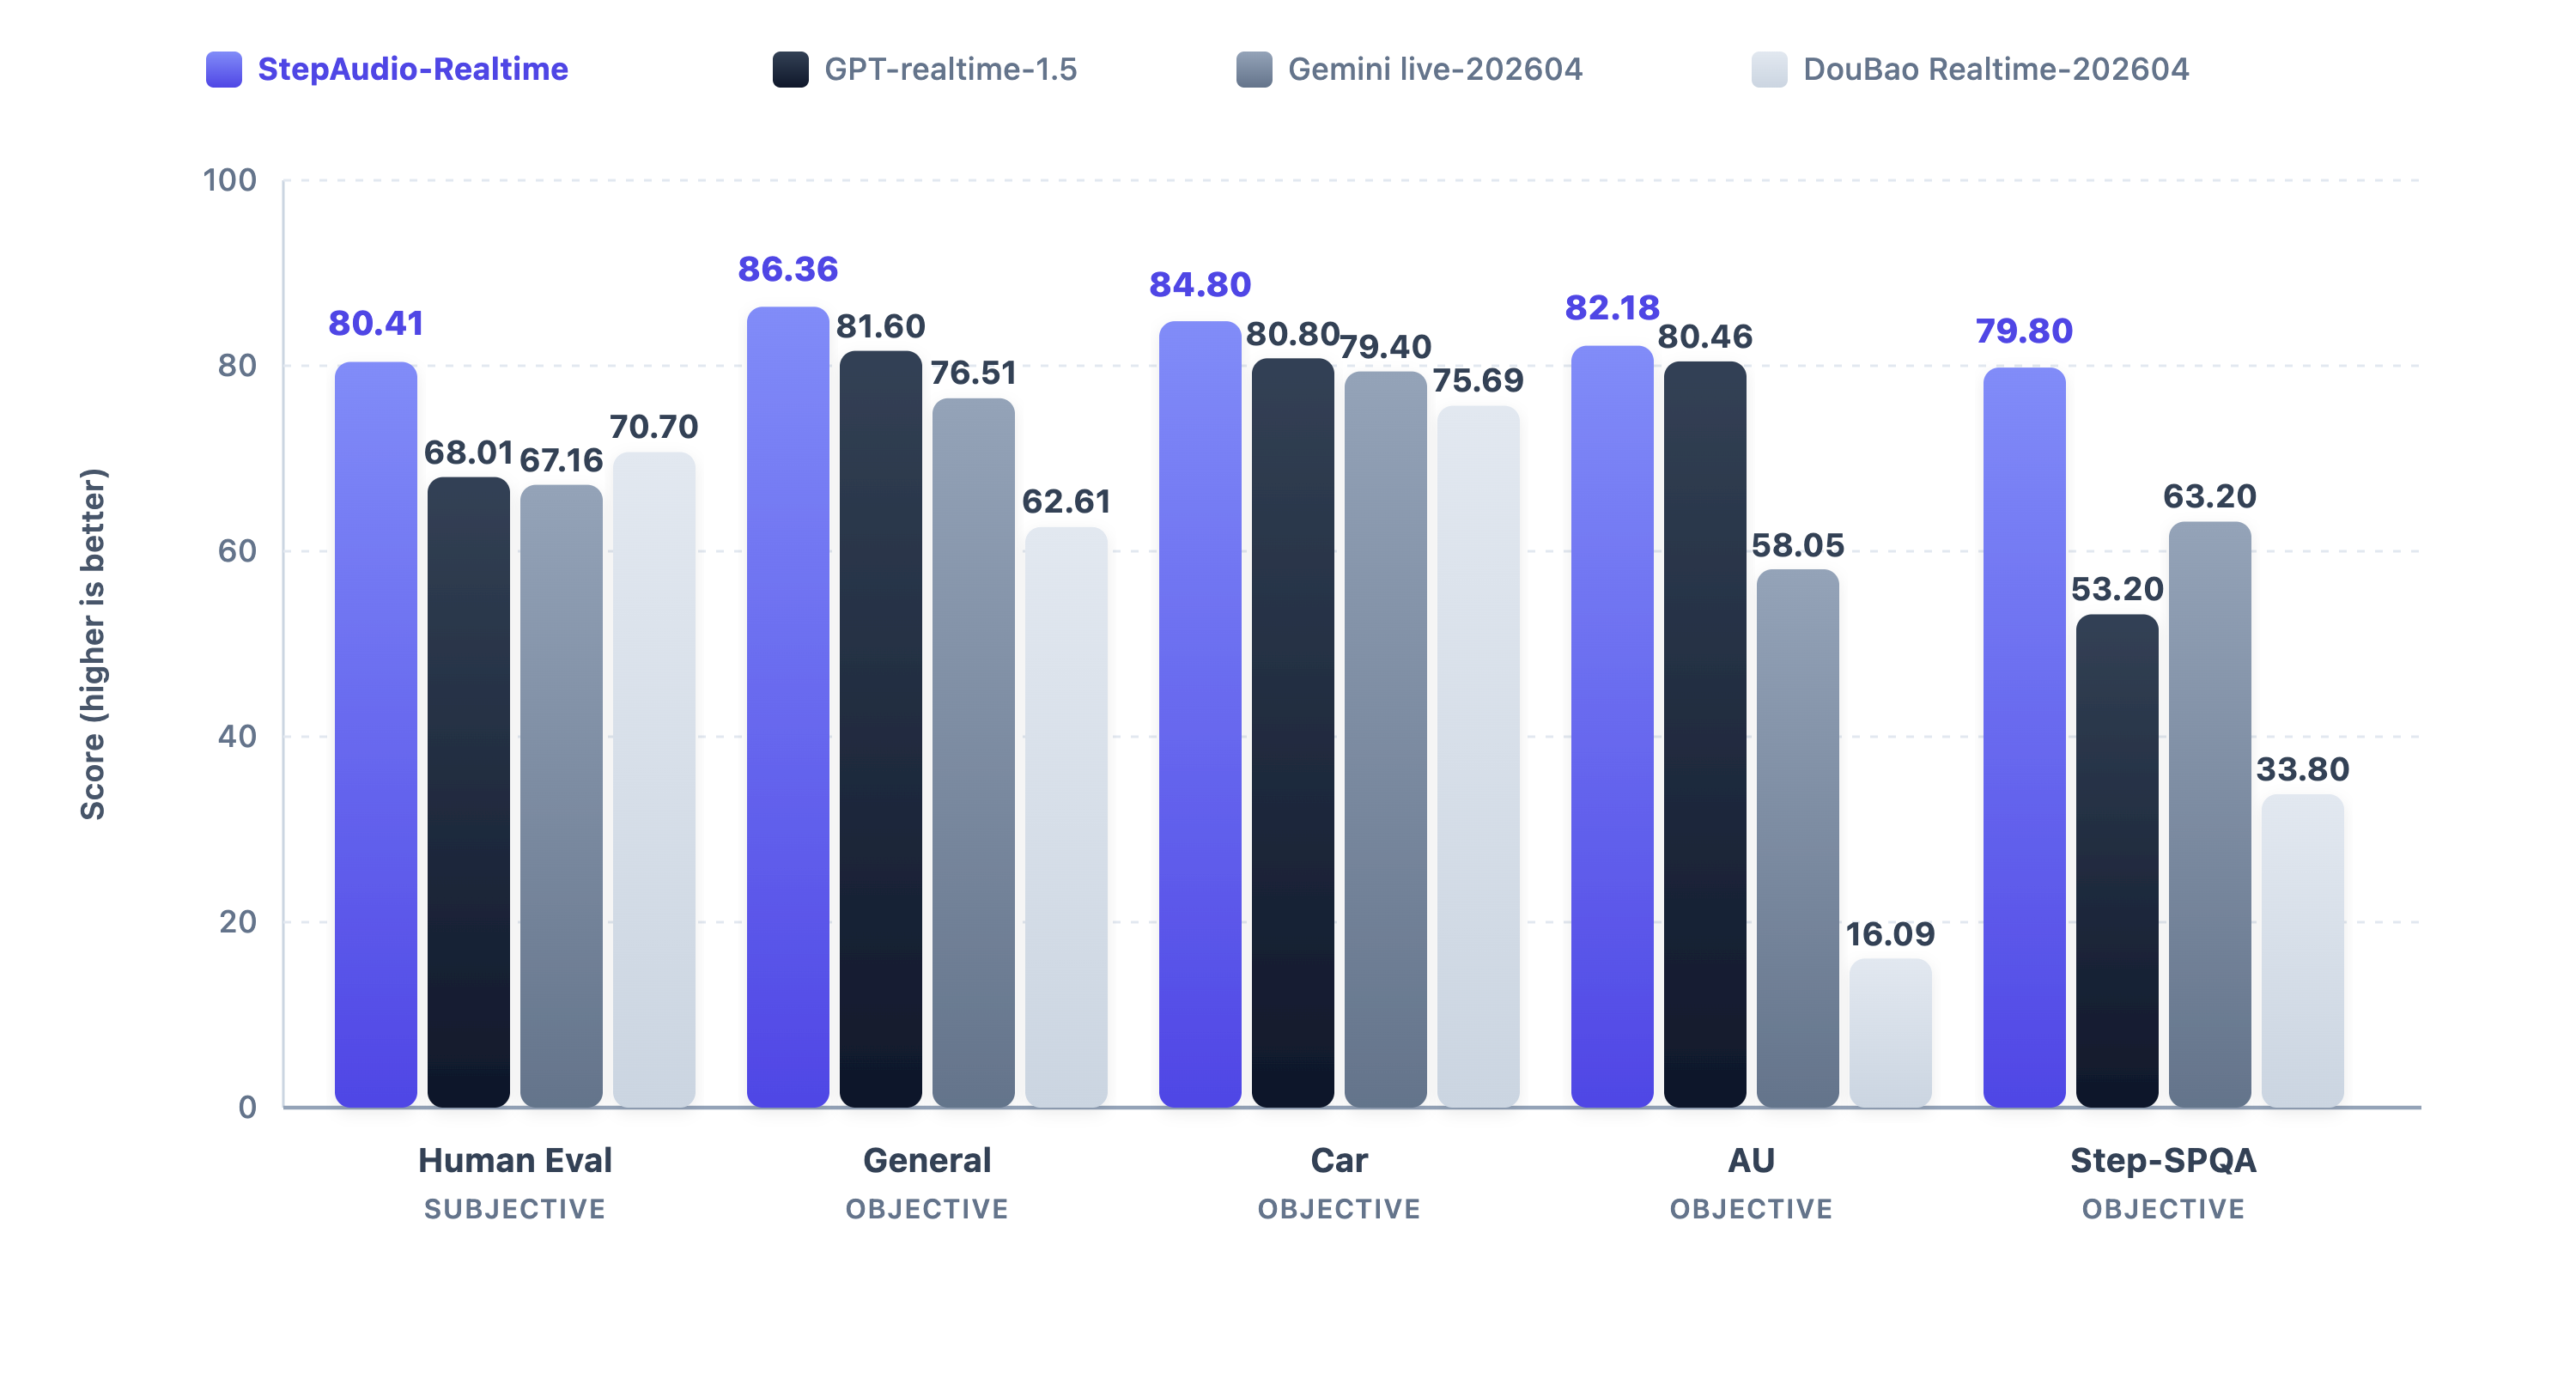
\includegraphics[width=1.0\linewidth]{figures/stepaudio25-realtime-evaluation.png}   
\caption{Realtime interaction evaluation. Higher is better. Best results are in bold.} 
\label{fig:realtime-eval}                                
\end{figure}  

\textbf{Results Analysis:}
As shown in Figure~\ref{fig:realtime-eval}, \steprealtime\ consistently outperforms competitive baselines across all five suites.
Notably, it achieves a +10.0 margin on the subjective human evaluation compared to the next-best system, validating the efficacy of our persona and naturalness conditioning. Furthermore, the +16.6 margin on Step-SPQA and strong performance on Step-Dialogue-Understanding indicate that the paralinguistic conditioning enhances acoustic comprehension without degrading general reasoning. The concurrent improvements in both subjective conversational quality and objective audio understanding demonstrate that our rehearsal schedule effectively balances specialized interaction training with foundational capabilities.
